\section*{Summary}
\subsection{Related Work}
    \begin{frame}
        Candoia draw inspiration from rich body of work
        \frametitle{Related Work}
         \begin{itemize}
            \item Platforms for reusing of tools and allow low cost addition of new tools
             \item Provides a repository of datasets from open-source repositories
         \end{itemize}
    \end{frame}

    \subsection{Platforms}
        \begin{frame}
            \begin{columns}
                \column{0.55\textwidth}
                    \textbf{Moose}
                    \begin{itemize}
                      \item A platforms for reusing of data mining tools.
                      \item Provides scripting and visualizations
                      \item Difference lies in the focus of the tools
                      \item Candoia is focused towards MSR and integrates MSR tools
                    \end{itemize}

                \column{0.55\textwidth}
                \textbf{RepoGrams}
                    \begin{itemize}
                      \item Helps researchers gather evaluation targets and calculate metrices on the target project
                    \end{itemize}
            \end{columns}
        \end{frame}

        \begin{frame}
            \begin{columns}
                \column{0.55\textwidth}
                    \textbf{Kenyon and Sourcerer}
                    \begin{itemize}
                      \item Defiens a databse schema for metadata and source code
                      \item Provide access to the dataset via SQL
                    \end{itemize}

                \column{0.55\textwidth}
                    \textbf{Alitheia Core}
                    \begin{itemize}
                      \item Provide a highly extensible framework for analyzing software product
                      \item Process metrics on a large database of open source projects source
                    \end{itemize}
            \end{columns}
         \end{frame}

        \begin{frame}
            \begin{columns}
                \column{0.55\textwidth}
                    \textbf{FLOSSMole}
                    \begin{itemize}
                      \item Analysis on the project metadata
                    \end{itemize}

                \column{0.55\textwidth}
                    \textbf{Groundhog}
                    \begin{itemize}
                      \item Infrastructure for downloading and analysing projects from SourceForge
                    \end{itemize}
            \end{columns}
        \end{frame}


    \subsection{Dataset}
        \begin{frame}
        \textbf{GHTorrent, PROMISE Repository, SourcererDB and Boa}
           \begin{itemize}
                \item Provides standard dataset for evaluation
                \item SourceDB also provides means to create custom dataset
            \end{itemize}
            Focus is on lifting the burden of data curation from user
        \end{frame}

\section{Summary and Future Work}

    \subsection{Summary}
        \begin{frame}
            \begin{figure}
                \centering
                    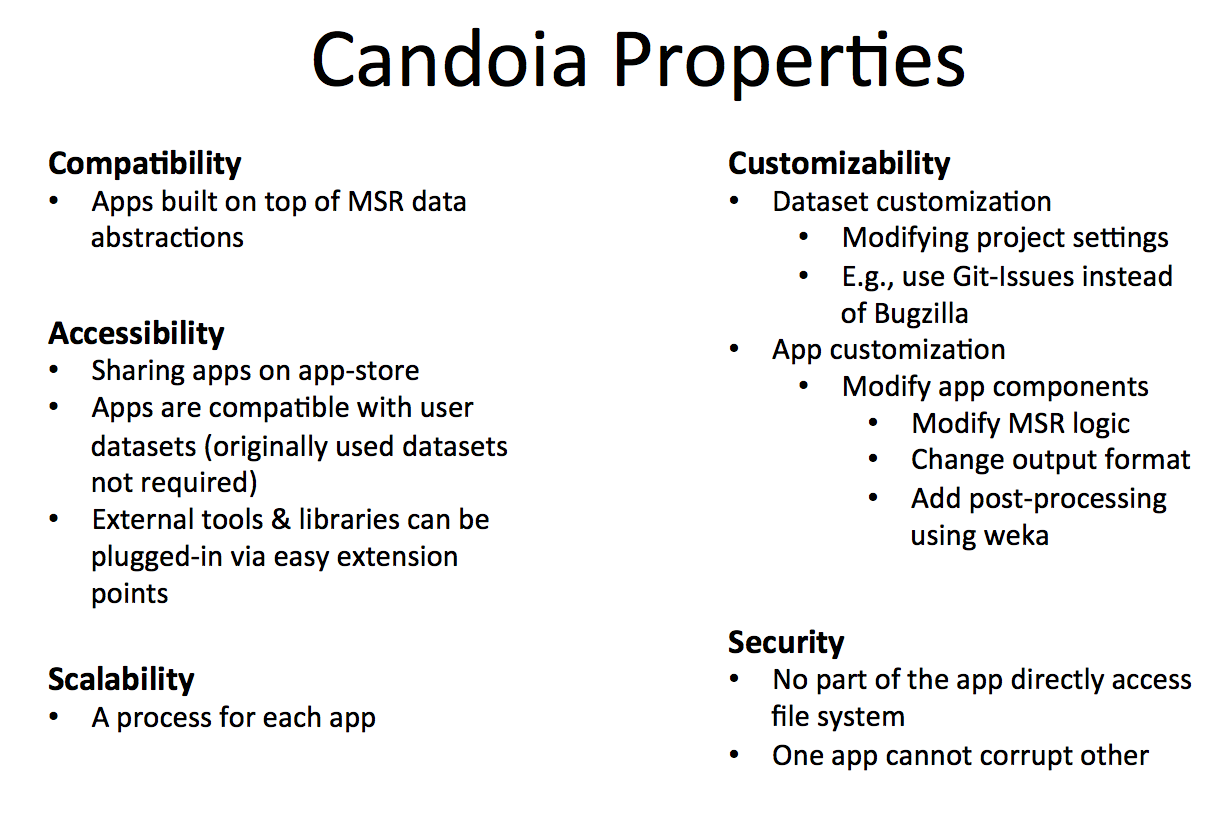
\includegraphics[scale=0.2]{figures/summary.png}
            \end{figure}
        \end{frame}


    \subsection{Future Work}
        \begin{frame}
            \frametitle{Future Work}
            \begin{itemize}
                \item Adding new software tools and technologies
                \item Building addiotional useful tools
                \item Utilizing underlying GPUs for better performance
            \end{itemize}
        \end{frame}

    \subsection{Acknowledgement}
        \begin{frame}
            \frametitle{Acknowledgement}
            \begin{itemize}
                \item This work was supported in part by the US National Science Foundation under grants CCF-15-18897, CNS-15-13263, and CCF-14-23370.
                \item  Dalton D. Mills and Trey Erenberger for helping with Candoia frontend implementation
                \item Eric Lin for implementing several Candoia apps
                \item Dr. Robert Dyer for valuable feedback
            \end{itemize}
        \end{frame}


        \begin{frame}
        \centering
            Candoia was awawrded distinguished poster\footnote{\tiny{\emph{Tiwari, Nitin M., Ganesha Upadhyaya, and Hridesh Rajan.
            "Candoia: a platform and ecosystem for mining software repositories tools.",
            ICSE'16}}}  at ICSE'16 \\

            \vspace{1cm}
            Full version of the work is appearing at MSR'17
             \footnote{\tiny{\emph{Tiwari, Nitin M., Ganesha Upadhyaya, Dr. Hoan Anh Nguyen and Hridesh Rajan.
                "Candoia: A Platform for Building and Sharing Mining Software Repositories Tools as Apps", MSR'17}}} \\
        \end{frame}

        \begin{frame}
            \centering
            Thank you
        \end{frame}


